\section{训练模型}
\label{sec:train-model}

\begin{frame}
  \begin{center}
    \Huge{\textcolor{red}{训练模型}}
  \end{center}

  \begin{enumerate}
    \item \alert{优化算法}
    \item \alert{工作流}
  \end{enumerate}    
\end{frame}

\subsection{优化算法}

\begin{frame}[fragile]{优化器}
  \begin{python} 
class Optimizer(object):
  def minimize(self, loss, var_list=None, global_step=None):
    grads_and_vars = self.compute_gradients(
      loss, var_list=var_list)
    return self.apply_gradients(
      grads_and_vars, 
      global_step=global_step)
  \end{python}
\end{frame}

\begin{frame}{RunStep过程}
  \begin{figure}
    \centering
    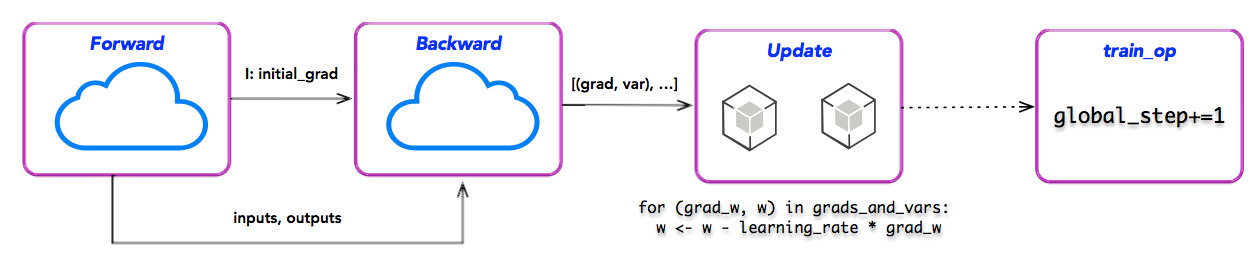
\includegraphics[width=1.0\textwidth]{bp-train-pipeline.png}
  \end{figure}
\end{frame}

\subsection{工作流}

\begin{frame}{工作流}
  \begin{figure}
    \centering
    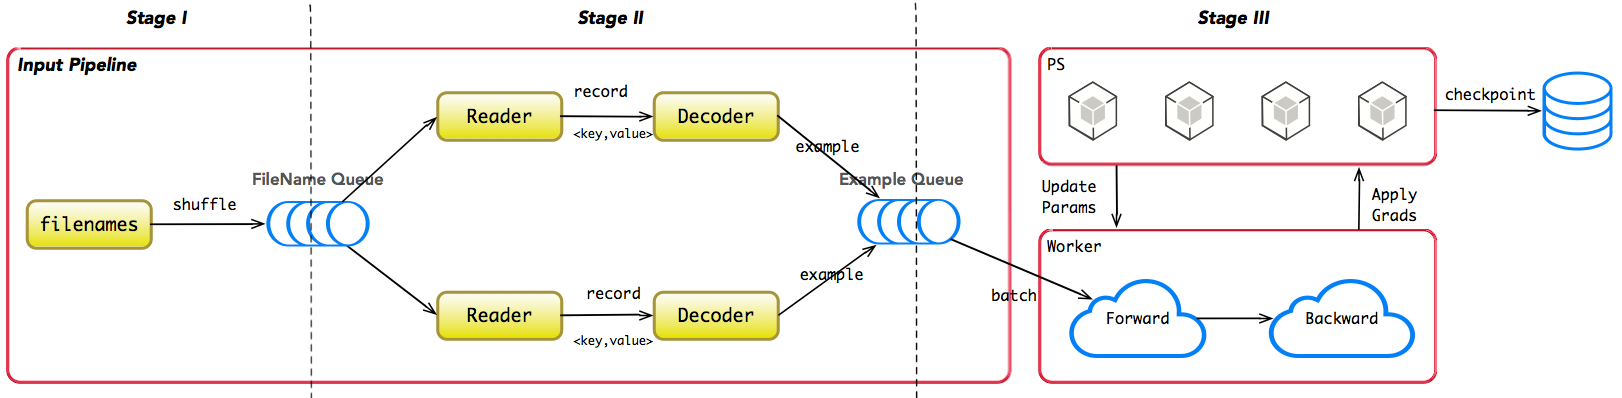
\includegraphics[width=1.0\textwidth]{tf-input-pipeline.png}
  \end{figure}
\end{frame}

\begin{frame}{协调协议}
  \begin{figure}
    \centering
    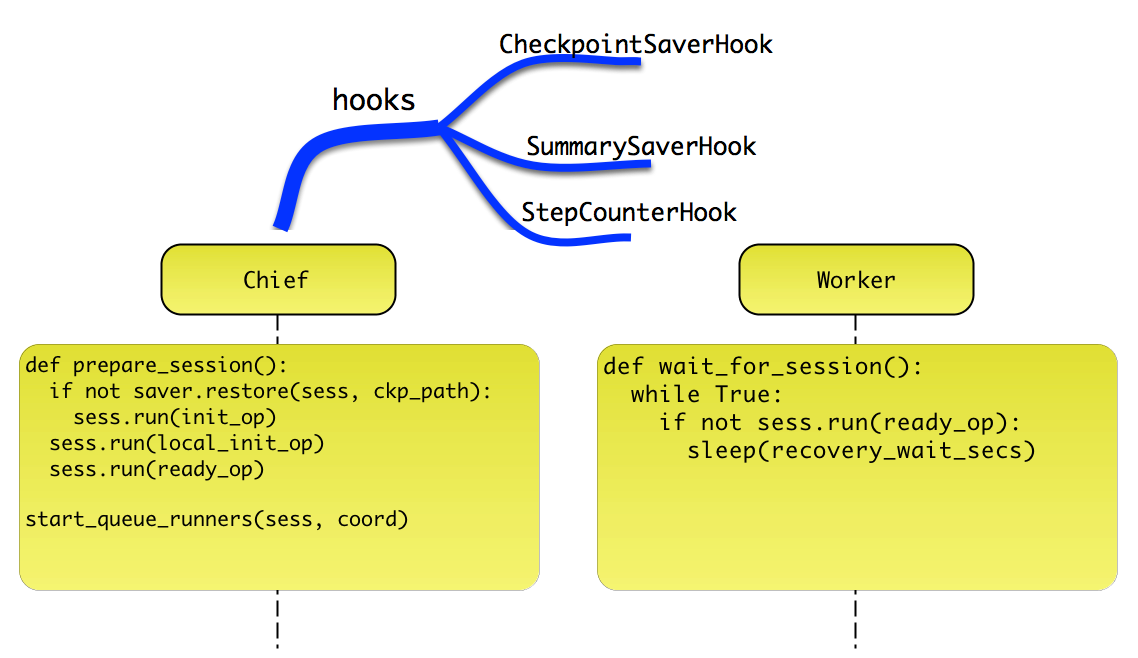
\includegraphics[width=0.8\textwidth]{py-train-chief.png}
  \end{figure}
\end{frame}
